%!TEX root = thesis.tex

\newpage

\chapter{Обзор реализованного программного обеспечения}

Для решения поставленной задачи в рамках данной работы было реализовано клиент-серверное приложение, позволяющее решать класс аналогичных по структуре задач. Для этого написаны несколько модулей, включающих в себя функционал, необходимый для решения конкретной подзадачи. Для удобства работы, каждый модуль имеет отдельные страницы, отвечающие за конкретные инструменты. Таким образом, весь процесс работы в приложении разбивается на несколько этапов, на каждом из которых решается конкретная подзадача. В данной работе можно выделить три этапа: первичный анализ данных, анализ остатков и вариограммный анализ. Далее в этой главе будут рассмотрены подробнее каждый из аспектов реализации.

Следует отметить, что каждая страница приложения имеет единый дизайн: экран можно условно поделить на панель выбора этапа анализа сверху и область исследования снизу. В свою очередь область исследования можно разделить также на две части: контрольная панель параметров и инструментов слева, и результаты вычислений и анализа справа. Любое изменение параметров контрольной панели сразу же отображается в качестве результата в области исследования.

\section{Модуль первичного анализа} % (fold)
\label{sec:mod_basis}

В \textbf{R} можно найти различные пакеты, позволяющие строить разнообразные гистограммы, диаграммы рассеяния, вероятностные графики, линейные графики, диаграммы диапазонов, размахов, круговые диаграммы, столбчатые диаграммы, последовательные графики и т.д., позволяющие увидеть специфику данных. В процессе реализации данной программы на языке \textbf{R} в качестве опорной литературы использовались источники \cite{Kabacoff2009R, Teetor2011RCook, Chang2012RGraph}.

\begin{figure}[ht]
\center{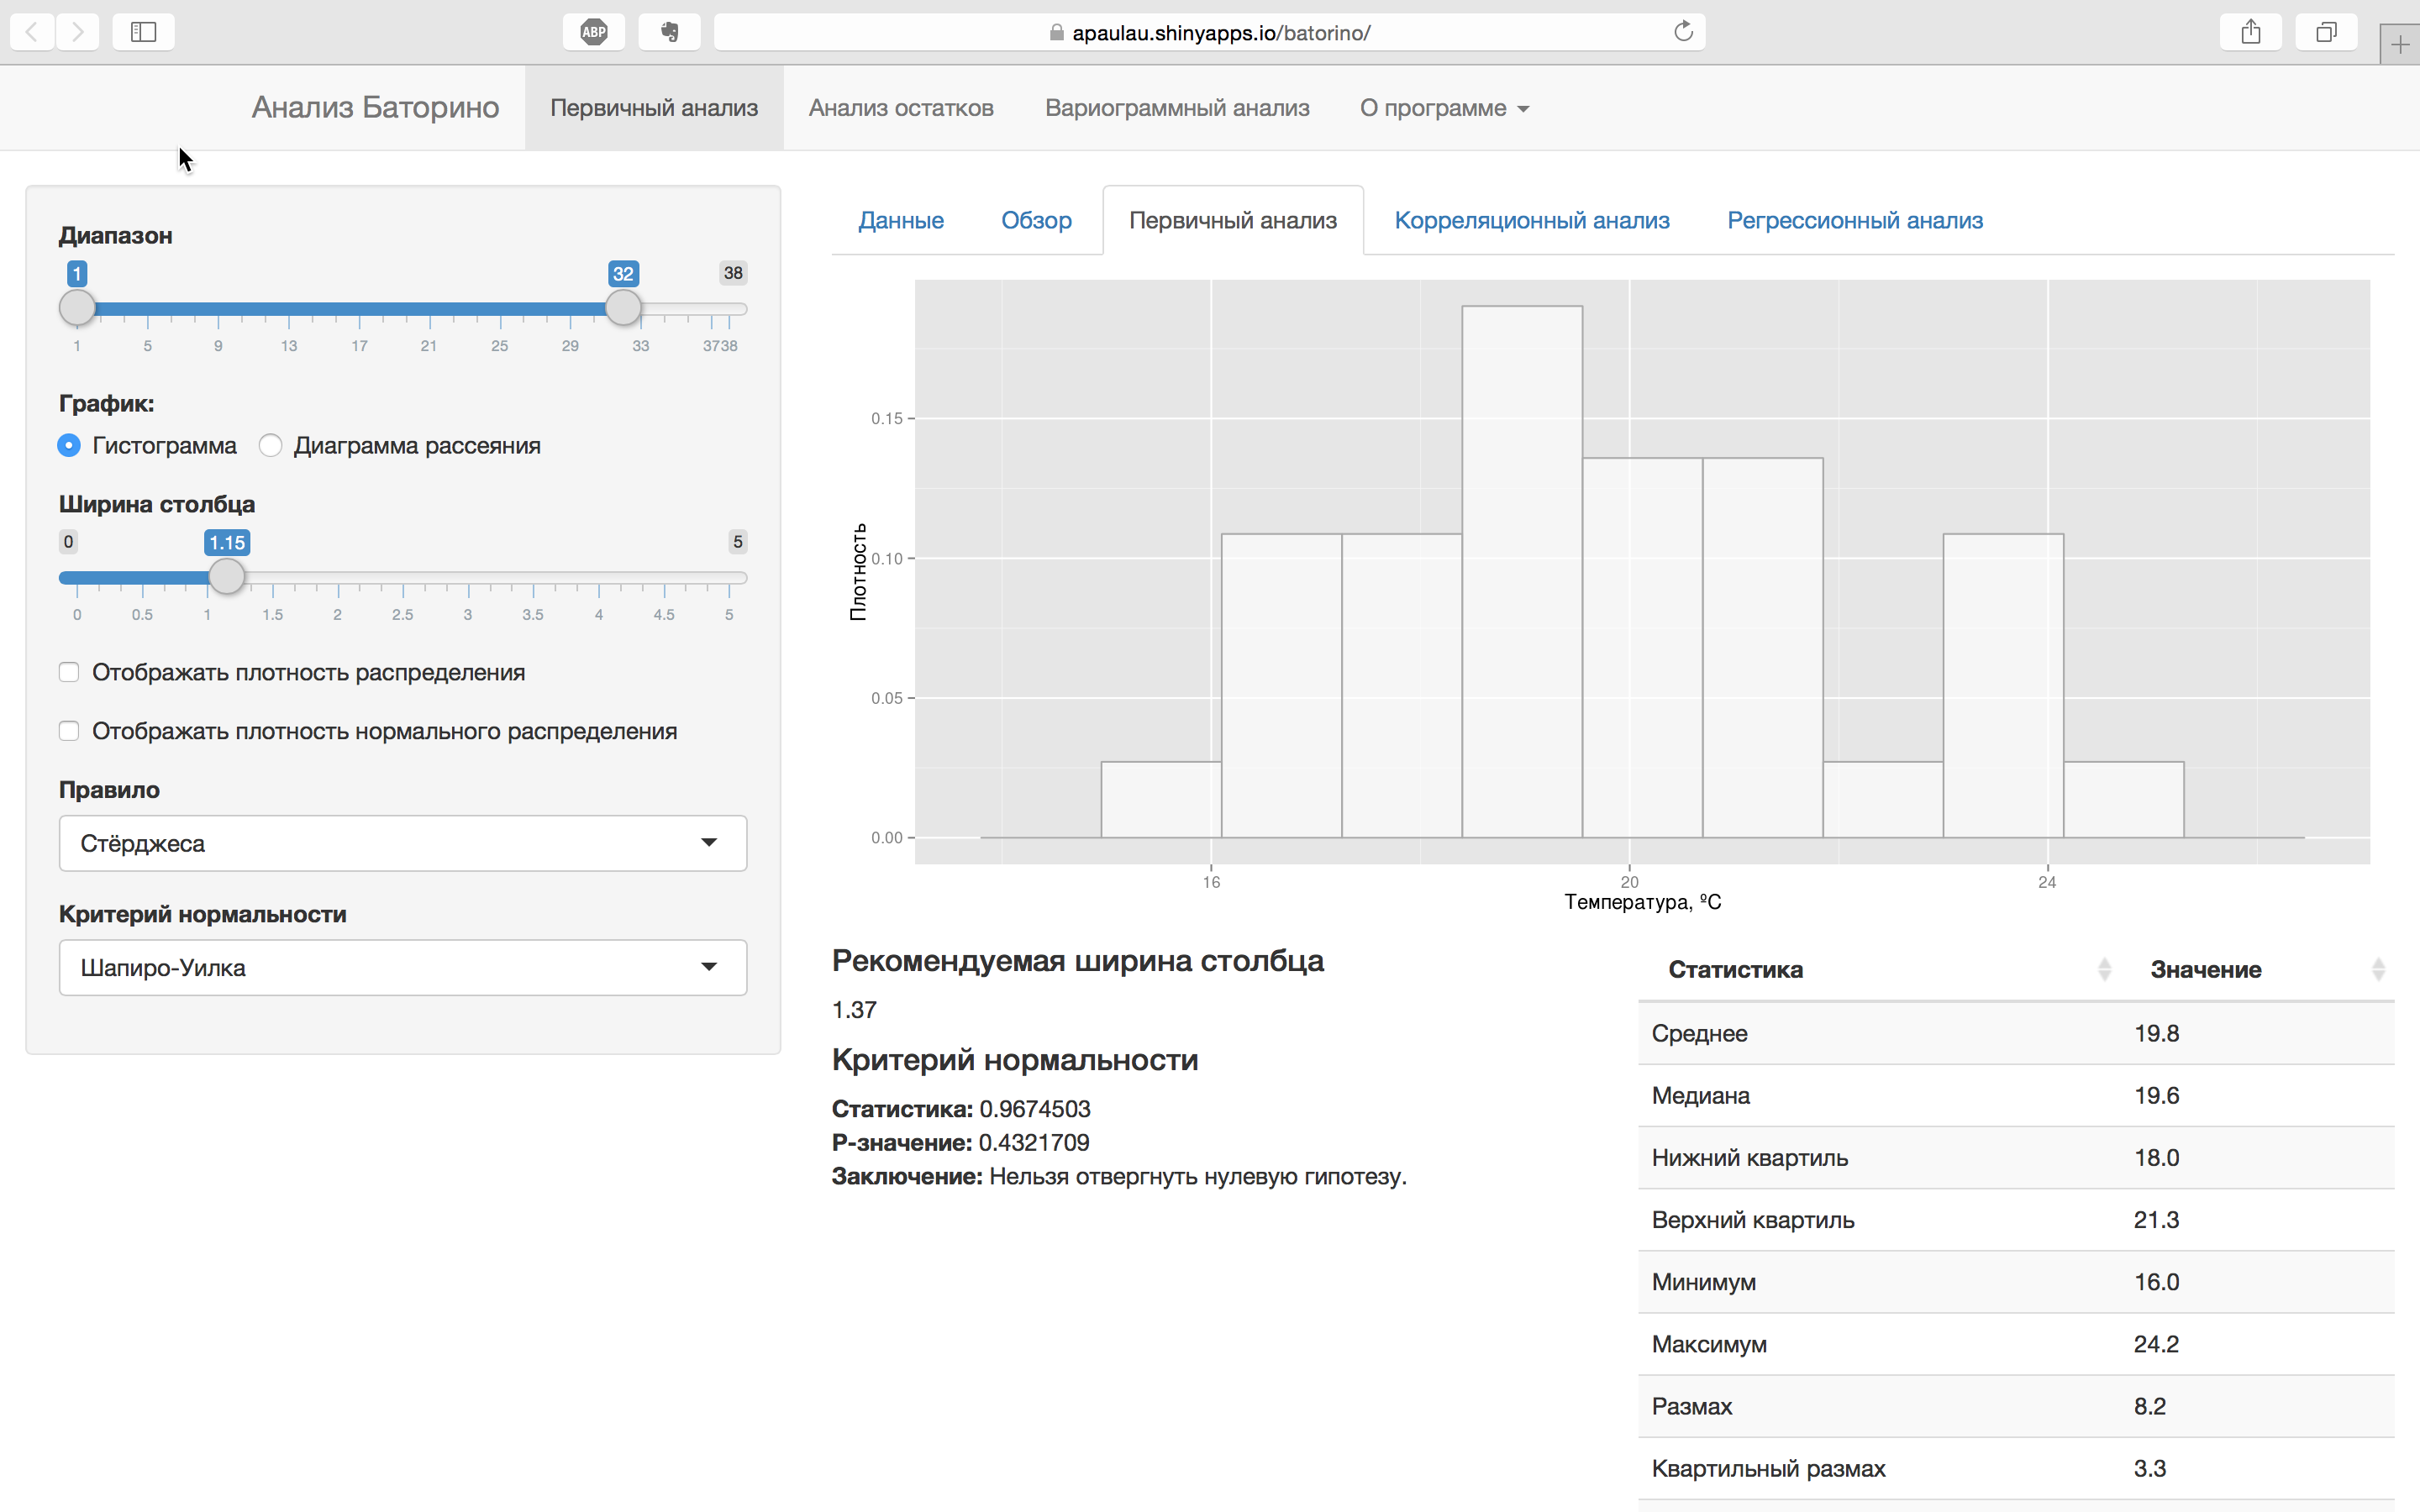
\includegraphics[width=1\linewidth]{../figures/static/1_basis.png}}
\caption{Первичный анализ и описательные статистики}
\label{img:mod_basis}
\end{figure}
Представленный модуль включает в себя возможности по просмотру и анализу данных: графически и с помощью таблицы, позволяющей сортировать и производить поиск по определённому признаку. На рисунке \ref{img:mod_basis} отображена вкладка первичного анализа, в которой представлены возможности по определению закона распределения исследуемых данных с помощью как проверки различными тестами, так и визуально с помощью гистограммы и графика квантилей. Контрольная панель позволяет изменять отображаемый в данный момент график, а также позволяет выбрать критерий нормальности. В случае выбора для отображения гистограммы, появляются управляющие элементы, позволяющие выбрать ширину столбца гистограммы и правило по её вычислению (например, правило Стерджеса), отобразить плотность выборочного распределения и кривую нормального распределения.

\textbf{R} предоставляет в пакете \textit{base} различные функции для расчетов базовых статистик. Также, в различных пакетах можно найти другие интересующие функции, как статистические, так и математические. Но в целях удобства, компактности и контроля за функциональностью на основе \cite{Eliseeva1995, Cramer1997} был разработан модуль \textit{dstats}, представленный в приложении \ref{c:listings} листинге \ref{lst:dstats}. Данный модуль позволяет вычислять все рассмотренные в данной работе описательные статистики, результат вычисления которых отображён на рисунке \ref{img:mod_basis} в виде таблицы.

Следующей вкладкой в данном модуле является корреляционный анализ. Данная страница позволяет оценить зависимость исследуемых данных с помощью диаграммы рассеяния, вычисляет коэффициент корреляции и с помощью критерия Стьюдента проверяет значимость коэффициента корреляции, а также вычисляет для него границы доверительного интервала. Среди прочего, данная страница содержит проверку на наличие выбросов с помощью критерия Граббса.

Вкладка регрессионного анализа (рисунок \ref{img:mod_regr}) позволяет получить регрессионную модель по исследуемым данным. График временного ряда содержит также линию регрессии.
\begin{figure}[ht]
\center{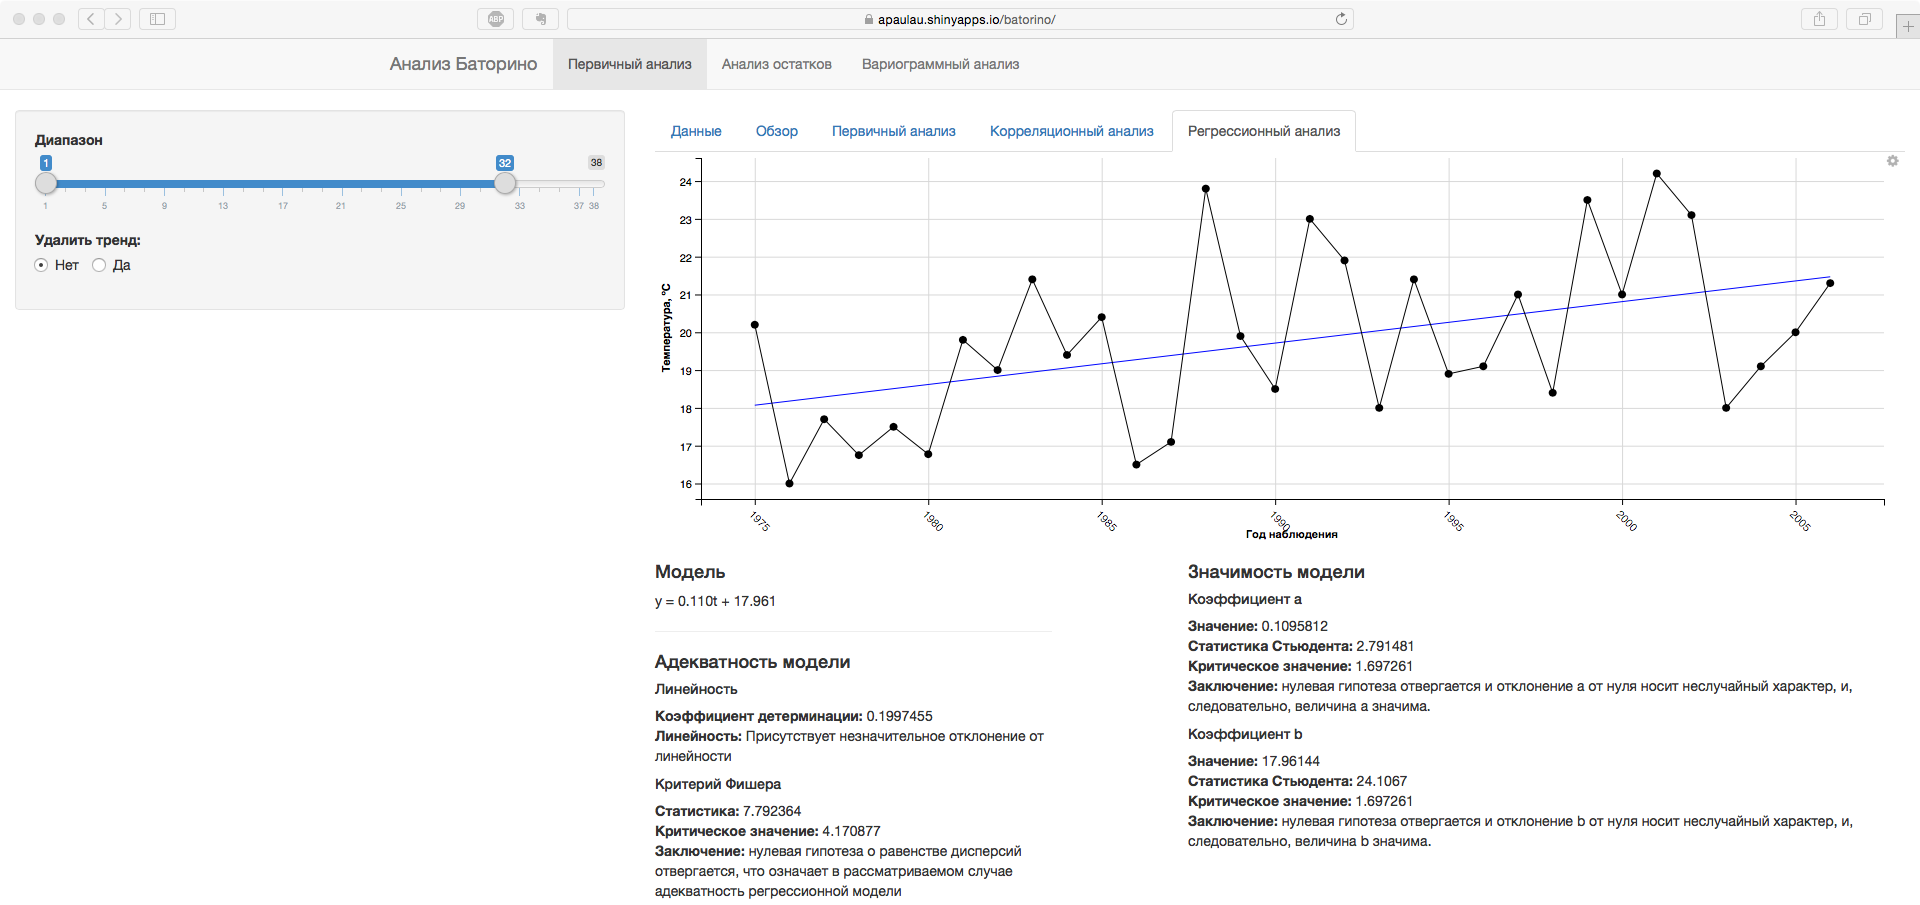
\includegraphics[width=1\linewidth]{../figures/static/2_regr.png}}
\caption{Регрессионный анализ}
\label{img:mod_regr}
\end{figure}
Представленная страница демонстрирует возможности по анализу вычисленной модели: определение значимости вычисленных коэффициентов, адекватность модели с помощью критерия Фишера и проверки линейности.

Инструменты, рассмотренные в рамках данного модуля, позволяют быстро получить информацию по исследуемым данным. А также сделать первые выводы и наметить шаги по дальнейшему исследованию. Заметим, что на каждом из этапов анализа и использования каждого из инструментов реализована возможность изменять объёмы выборки, отбрасывая первые или последние элементы. Это позволяет быстро оценить, насколько влияют данные на результат в конкретном случае.

% section mod_basis (end)

\section{Модуль анализа остатков} % (fold)
\label{sec:mod_residuals}

Модуль анализа остатков является логическим продолжением рассмотренного ранее. После регрессионного анализа и удаления из исходного временного ряда тренда, основанного на регрессионном уравнении, получаем ряд остатков. Для его анализа реализованы возможности, которые включают в себя некоторые возможности предыдущего модуля. Исключение составляют инструменты регрессионного и корреляционного анализов. Поскольку исследуемый на данном этапе временной ряд представляет собой ошибку.

Таким образом, данный модуль позволяет проверить остатки на нормальность как с помощью графиков квантилей и гистограммы, так и различными критериями: Шапиро-Уилка, $ \chi^2 $-Пирсона, Колмогорова-Смирнова. В дополнение к этому имеется возможность проанализировать описательные статистики, а также исследовать автокорреляционную функцию. Страница с таким инструментом представлена на рисунке \ref{img:mod_acf}.
\begin{figure}[ht]
\center{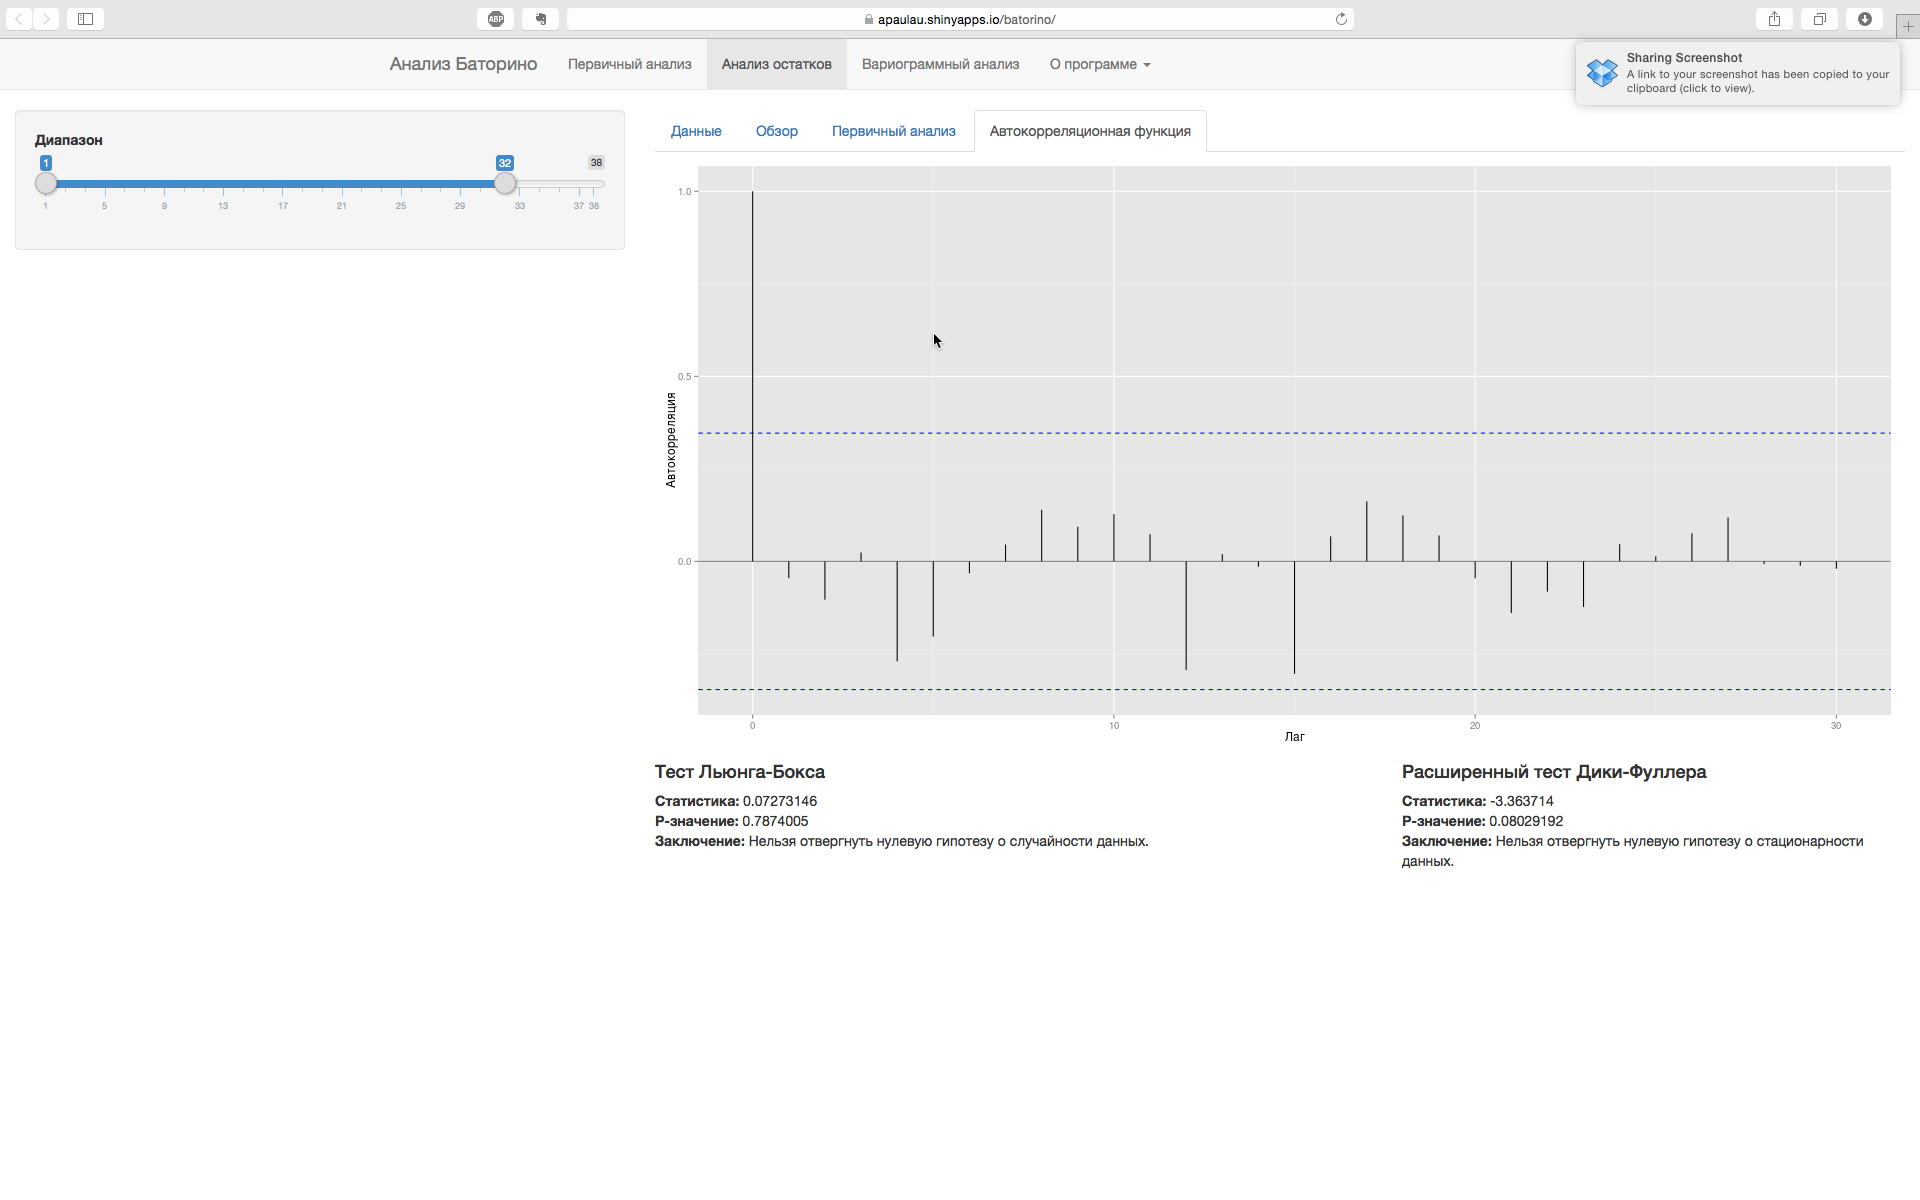
\includegraphics[width=1\linewidth]{../figures/static/3_acf.png}}
\caption{Анализ автокорреляционной функции}
\label{img:mod_acf}
\end{figure}
На рисунке продемонстрирован график автокорреляционной функции, позволяющий визуально определить наличие автокорреляций в исследуемых данных. Также проверить наличие значимых автокорреляций позволяет реализованный тест Льюнга-Бокса. В свою очередь, расширенный тест Дики-Фуллера, также представленный на рассматриваемой странице, проверяет наличие стационарности в исследуемом временном ряду.

В зависимости от результатов, полученных на рассмотренном этапе, можно либо закончить исследование, либо продолжить в модуле вариограммного анализа. Закончить исследование стоит в том случае, если модель удовлетворительного качества, либо в случае, когда не выполняются условия для проведения следующего этапа.

% section mod_residuals (end)

\section{Модуль вариограммного анализа} % (fold)
\label{sec:mod_variogram}

В данном модуле используются современные геостатистические методы и инструменты, которые, в рамках \textbf{R}, реализованы пакетом \textit{gstat}. В этом пакете представлены функции для вычисления вариограмм, подбору моделей и параметров, интерполирования методами кригинга и методы валидации конечных результатов. Интерполирование методами кригинга подразумевает наличие ряда моделей вариограмм, поэтому в рассматриваемом модуле акцент сделан именно на подборе и анализе моделей вариограмм, наиболее подходящих для экспериментальных данных.

Начальный шаг состоит в подборе модели и её параметров к экспериментальной вариограмме. Для построения экспериментальной вариограммы присутствует возможность использовать две разновидности оценок вариограммы: рассмотренная в главе 2 оценка Матерона и робастная оценка Кресси-Хокинса \cite{cressie1993statistics}. Для подбора модели вариограммы, в общем случае, существует два подхода: подбор визуально силами исследователя, и автоматическими методами. В данном модуле в полной мере реализованы оба подхода. В первом случае, изменение любого из параметров модели позволяет незамедлительно оценить эффект как на графике семивариограммы, так и по конечному прогнозу кригингом.

\begin{figure}[ht]
\center{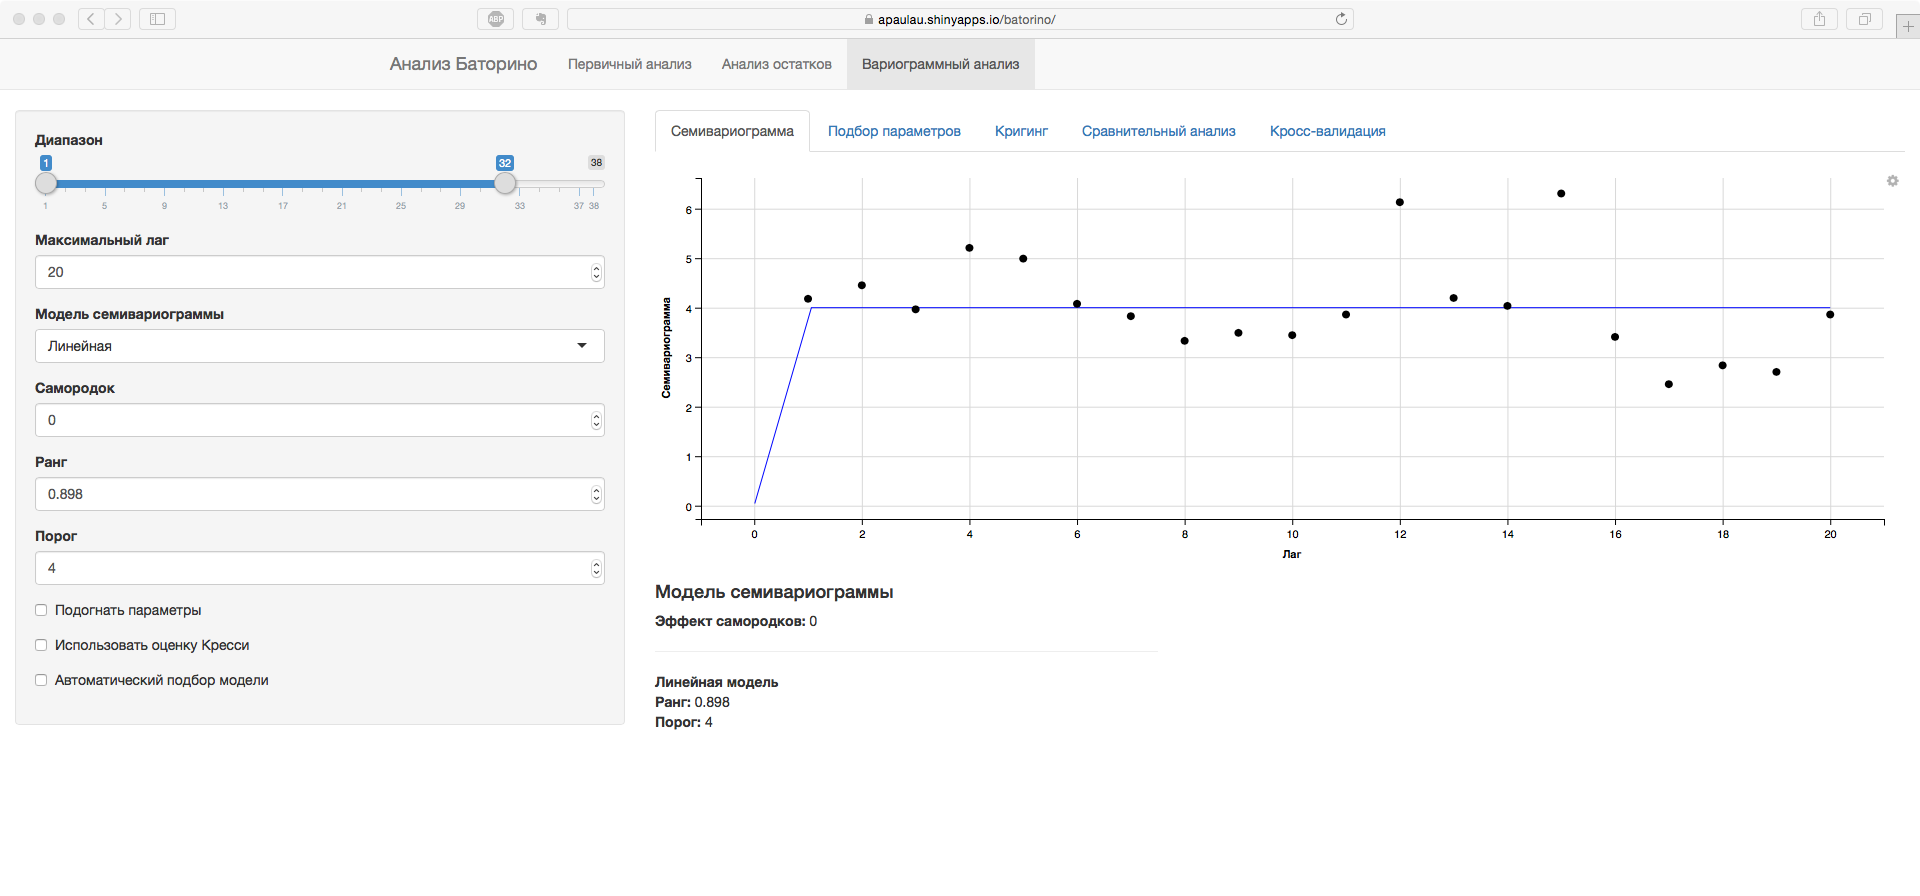
\includegraphics[width=1\linewidth]{../figures/static/4_variogram.png}}
\caption{Возможности по подбору модели семивариограммы}
\label{img:mod_variogram}
\end{figure}
На рисунке \ref{img:mod_variogram} изображён скриншот начального этапа вариограммного анализа. Инструменты данной страницы позволяют выбрать модель из следующих: Линейная, Сферическая, Экспоненциальная, Гауссовская, Круговая, Бесселя, Пентасферическая, Волновая, Логарифмическая. А также задать к выбранной модели параметры. Заданные параметры считаются начальными, если выбрать опцию подгона методом наименьших квадратов.

На этом шаге также можно воспользоваться реализованным в рамках данной работы алгоритмом автоматического подбора модели. Данная функциональность позволяет сразу перейти к вычислению прогнозных значений и не требует каких-либо прикладных знаний у пользователя. Алгоритм заключается в переборе всех представленных в пакете \textit{gstat} моделей, и подборе параметров с помощью функции \textit{fit.variogram} из того же пакета. Каждая итерация сопровождается оптимальным набором параметров для конкретной модели и невязкой между экспериментальной семивариограммой и моделью. Выбор наилучшей модели осуществляется по минимальному значению невязки. Представленная страница позволяет оценить по графику семивариограммы подобранные либо вручную, либо автоматически модель и параметры.

При использовании той или иной модели интерполяции крайне важно правильно подобрать значения модельно-зависимых параметров. Для кригинга такими параметрами являются параметры модели семивариограммы. Для проверки качества модели в дальнейшем используется кросс-валидация. Кросс-валидация является наиболее простым и часто использующимся подходом при сравнении результатов, получаемых различными методами или одним и тем же методом, но с различными параметрами. В данном случае процесс кросс-валидации заключается в последовательном исключении одного значения температуры из исследуемых данных $ \varepsilon(t) $ и построении интерполяции в этой точке по валидируемой модели. Таким образом, получаем ряд интерполяций $ \varepsilon^{*}(t) $, который должен в идеальном случае воспроизводить поведение исследуемого ряда. По ряду $ \varepsilon^{*}(t) $, с помощью различных статистик можно оценивать качество конкретной модели семивариограммы. С помощью таких статистик можно проследить, как изменяется качество модели при изменении какого-либо из параметров. В данной работе используются следующие статистики \cite{saveliev2012}:
\begin{enumerate}
	\item Сумма квадратов невязок:
	\begin{equation*}
		S = \sum_{i = 1}^{n} (\varepsilon(t_i) - \varepsilon^{*}(t_i))^2,
	\end{equation*}
	где $ n $ --- объём выборки.
	\item Коэффициент эффективности:
	\begin{equation*}
		E = \frac{S}{\sum_{i=1}^{n}(\varepsilon(t_i) - \bar{\varepsilon})},
	\end{equation*}
	где $ \bar{\varepsilon} $ --- среднее значение исследуемых данных.
	\item Среднее абсолютных значений:
	\begin{equation*}
		MAE = \frac{1}{n} \sum_{i=1}^{n} | \varepsilon(t_i) |,
	\end{equation*}
	где $ n $ --- объём выборки.
	\item Среднеквадратическая ошибка
	\begin{equation}
	\label{eq:mse}
		MSE = \frac{1}{n} \sum_{i=1}^{n} (\varepsilon(t_i) - \varepsilon^{*}(t_i))^2,
	\end{equation}
	где $ n $ --- объём выборки.
	\item Коэффициент корреляции $ r_{\varepsilon\varepsilon^{*}}. $
\end{enumerate}

Следующая вкладка (рисунок \ref{img:mod_fit}) заключает в себя функциональность по подбору параметров.
\begin{figure}[ht]
\center{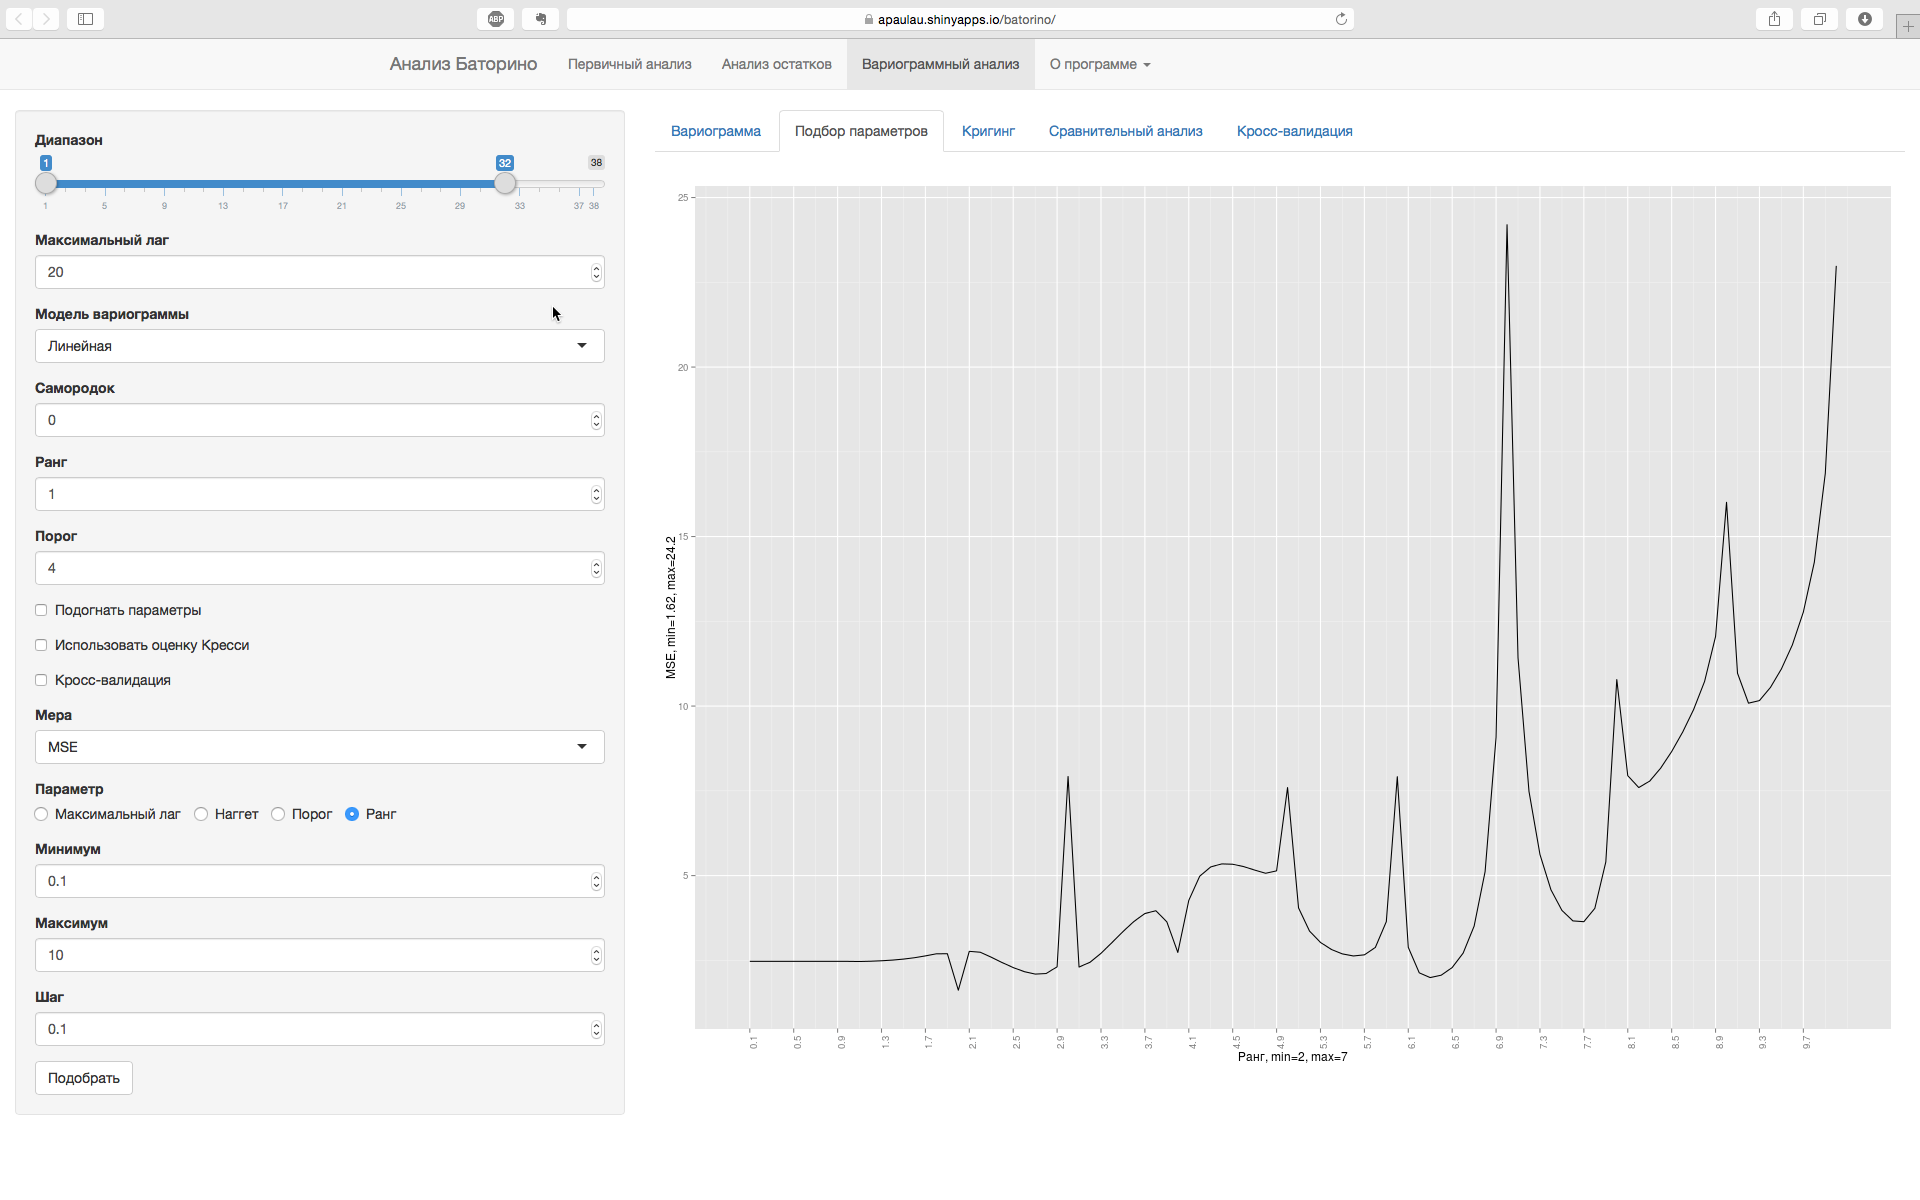
\includegraphics[width=1\linewidth]{../figures/static/5_fit.png}}
\caption{Подбор параметров модели семивариограммы}
\label{img:mod_fit}
\end{figure}
В большей мере это относится к ручному выбору. В общем случае, подбор осуществляется следующим образом:
\begin{itemize}
	\item задаются вид модели семивариограммы, начальные значения параметров и статистика
	\item выбирается параметр для подбора, диапазон поиска и шаг итерации
	\item на каждом шаге кригингом вычисляются прогнозные значения
	\item на основе полученных прогнозных значений строится выбранная статистика
\end{itemize}
В результате такого процесса получается ряд оценок моделей, из которых выбирается оптимальная. Затем процесс повторяется для другого параметра и так далее, пока не найдётся оптимальная модель.

В реализованном приложении имеется два подхода по оценке качества построенной модели. Используя первый подход, перекрёстный, модель оценивается с помощью описанного ранее метода кросс-валидации. При втором подходе, адаптивном, в исследуемых данных отдаётся предпочтение последним наблюдениям. Для этого из исходных данных исключается некоторое количество значений и модель строится по оставшимся. Подбор параметров осуществляется по показателям качества, основанным на отклонении вычисленных значений от исключенных. Таким образом, как будет показано в главе 4, достигается наилучший прогноз в краткосрочной перспективе.

Таким образом на данной странице можно оценить поведение модели при изменении какого-либо из параметров и для каждого подобрать оптимальное значение.

Страница кригинга (рисунок \ref{img:mod_krige}) является наглядной демонстрацией применения всего вышеописанного. На ней изображается график с наблюдаемыми значениями и прогнозными значениями, вычисленными по линейной регрессионной модели и кригингом.
\begin{figure}[ht]
\center{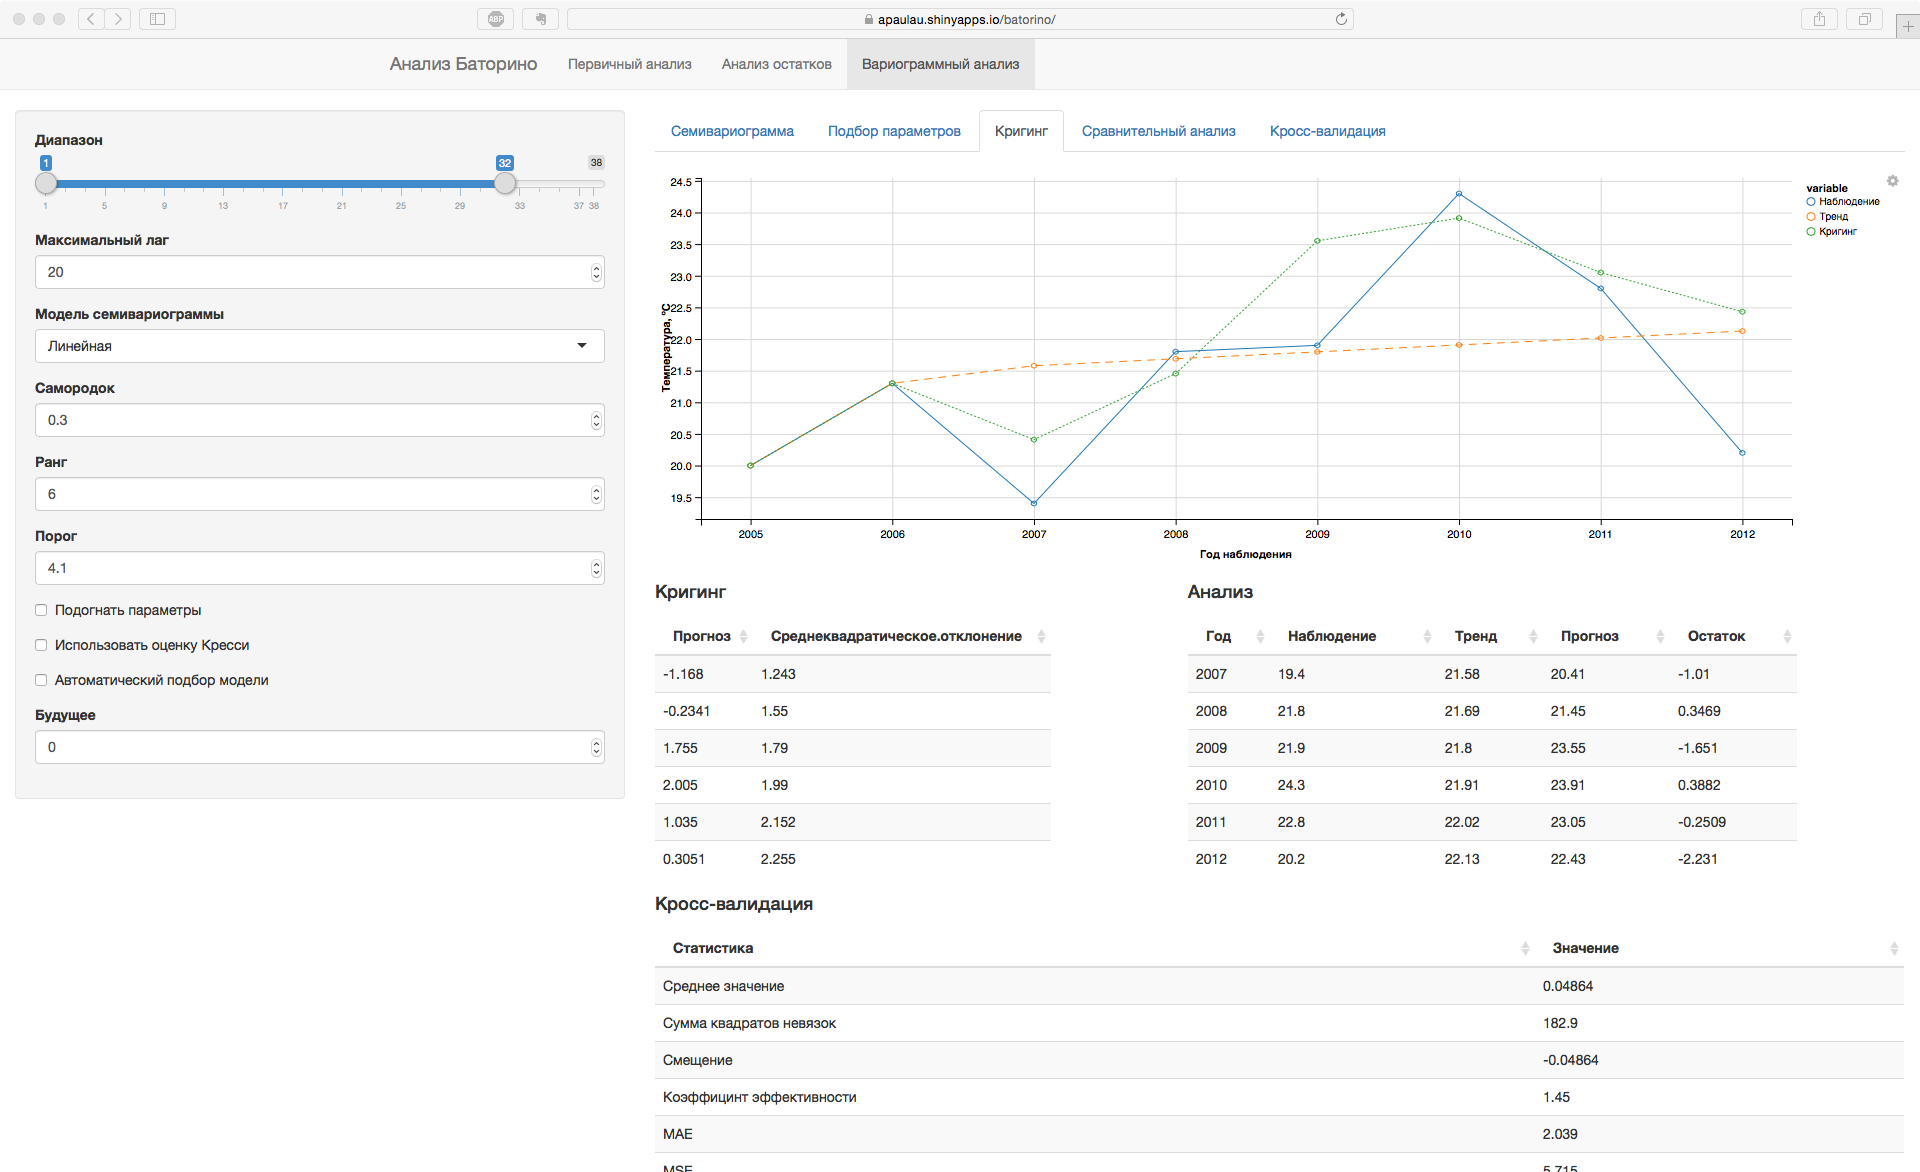
\includegraphics[width=1\linewidth]{../figures/static/6_krige.png}}
\caption{Сравнение прогнозных значений}
\label{img:mod_krige}
\end{figure}
Это позволяет оценить полученную модель и сделать конкретные заключения. Приводятся вспомогательные таблицы с произведёнными в процессе расчётами. В первую очередь это результаты кригинга со среднеквадратической ошибкой для каждого из значений. Также отображается табличный вариант данных, изображённых на графике. И последняя таблица показывает значения показателей качества после применения кросс-валидации, что сразу позволяет сравнить конкретную модель с другими.

% section mod_variogram (end)